\chapter{Fundamentos Teóricos}
\label{c:fundamentosteoricos}

\vspace{1cm}

En este capítulo se presentan los principales fundamentos teóricos para llevar a cabo el presente trabajo.

Primeramente se describen las operaciones morfológicas: conversión a escala grises sobre una imagen, erosión, dilatación, bounding box y convex hull.

Luego, se presentan los conceptos más importantes de las características locales junto con sus propiedades más significantes como así también una distinción de los los detectores dependiendo del uso de los mismos. Además, se hace una breve síntesis de las características locales junto a sus propiedades más importantes con una discusión sobre las mismas.

Finalmente, se detalla los fundamentos de un método de detección características, haciendo incapie en método SURF y su relación con SIFT. Además, se describe la correspondencia de características entre imágenes mediante  la búsqueda del vecino más cercano ayudado del método estadístico RANSAC para la eliminación de correspondencias espurias.

% http://opencv.willowgarage.com/documentation/cpp/geometric_image_transformations.html
\newpage

\subsection{otra cosa}
      En este trabajo, nos enfocaremos en un detector y descriptor invariante a escala y en el plano. Tanto el detector como el descriptor no utilizarán información de color, sino que se valdrán de una imagen en escala de grises para llevar a cabo el procedimiento. Estos, parecen ofrecer un buen compromiso entre la complejidad de las características y la robustez a las deformaciones que comúnmente ocurren. La distorsión o torcimiento, escalado no isótropo\footnote{En geometría euclídea, el \textbf{Escalado uniforme} o \textbf{Escalado isótropo} es una transformación lineal que incrementa o decrementa un objeto por un factor de escala el cual es el mismo en todas las direcciones. El resultado del escalado, es similar (en sentido geométrico) al original. Si se utiliza al menos un factor de escala diferente para un eje de coordenadas, se está en presencia de un \textbf{Escalado no uniforme} o \textbf{Escalado no isótropo} resultando en un cambio en la forma del objeto.} y efectos de la perspectiva se asumen que son alteraciones de segundo orden que son cubiertos en cierto grado por la robustez general del descriptor seleccionado.

      Un detector de puntos de interés usado recientemente es el Detector rápido de características robustas o SURF (Speeded Up Robust Features) \cite{citeulike:9456628, citeulike:7676197, Bay:2008:SRF, bb53077, TuytelaarsM07, Bay:2008:SRF, BouGar}. El método SURF es un detector y descriptor invariante a escala y rotación (logrado mediante la asignación de una orientación a cada punto clave detectado) que posee buenas propiedades de repetibilidad, distintividad y robustez permitiendo además calcularse y ser comparado rápidamente respecto a otros métodos. El mismo está basado en conceptos del algoritmo de Transformación de características invariante a la escala o SIFT (Scale Invariant Feature Transform) \cite{citeulike:3484001, citeulike:9456628, citeulike:7676197, bb53077, journals/tvcg/WagnerRMDS10, TuytelaarsM07, bb48614, Nixon:2002:FEI, BouGar, 5739718, conf/ismar/2004}. 
      -------------
      Como se mencionó anteriormente, el algoritmo SURF define la localización y escala para cada una de las características detectadas. Este factor de escala, puede ser usado para definir el tamaño de una ventana alrededor de cada punto característico, de tal manera de poder definir un área vecina que incluya la misma información visual, sin importar la escala en que el objeto fue fotografiado. Así, esta información visual incluida en esa vecindad, resulta útil para caracterizar el punto clave y ayuda en la distinción del mismo de otros similares.

      Para describir el área vecina de los puntos característicos, se usan descriptores de características, que usualmente (en el caso de comparación entre imágenes) son vectores N-dimensionales que resultan ser invariantes a cambios de iluminación y a pequeñas deformaciones de perspectivas (en el caso ideal). Además, resultan potencialmente usables para ser comparados mediante el uso de una métrica de distancia, como por ejemplo: la distancia euclídea. 

      En el caso del algoritmo SURF, el descriptor por defecto posee 64 elementos (SIFT utiliza 128) y este vector caracteriza el patrón de intensidad en el área que rodea a un punto característico. Cuanto más similares sean dos puntos característicos, más cercanos serán sus vectores descriptores. 

      Así, dadas dos imágenes de la misma escena, primeramente se extraen los puntos claves y los descriptores asociados con cada uno de ellos para ambas imágenes. Luego, cada vector descriptor en la primer imágen es comparado con todas los vectores descriptores de la segunda imágen. El par que obtiene la menor distancia entre ellos, es considerado la mejor coincidencia para dicha característica. Luego el proceso es repetido para todas las características de la primer imágen. Este esquema básico para coincidencias es conocido como coincidencias por fuerza bruta. El método termina considerando los 25 más cercanos y los demás pares son descartados.

\section{Pasos para implementación del algoritmo SURF}
\begin{itemize}
 \item Se toma una imagen del objeto a detectar y se detectan los puntos claves junto con sus descriptores asociados. Es importante que esta imagen contenga solo el objeto a detectar. Dicha detección se realizan mediante SURF cuyos pasos pueden resumirse:%\footnote{\url{http://robocv.blogspot.com.ar/2012/02/real-time-object-detection-in-opencv.html}}:
  \begin{enumerate}
    \item Busca puntos interesantes en la imagen usando matrices hessianas.
    \item Determina una orientación para cada punto encontrado.
    \item Usa wavelets haar en una región cuadrada orientada alrededor del punto clave para buscar los gradientes de intensidad en la dirección $x$ e $y$. Esta región cuadrada es dividida en 16 sub regiones, y cada sub región construye 4 características (que son básicamente sumas de cambios de gradientes), resultando el descriptor surf en un vector de 64 dimensiones.
  \end{enumerate}
 \item Se repite el paso anterior para cada fotograma capturado por la cámara.
 \item Se emplea la la estrategia de correspondencias para buscar las coincidencias validas.
 \item Para obtener un bounding box alrededor del objeto detectado, las coincidencias validas, se busca la homografía que transforma los puntos de la imagen de entrenamiento a la imagen objetivo. Usando esta homografía, se transforman las 4 esquinas de la imagen de entrenamiento y se coincideran estos 4 puntos como vertices y dibujar una caja en el frame de video. Se dibuja la caja solo si se encuentran 4 o más buenos macheos.
\end{itemize}

\section{Filtrado de imágenes}
El filtrado es una de las principales tareas en el procesamiento de imágenes y de señales. Es un proceso que busca extraer ciertos aspectos de la imágen que resultan ser información conveniente o importante en el contexto de una aplicación dada. El filtrado, remueve ruido, extrae características visuales interesantes, permite el escalado de imágenes, etc.

Caundo miramos una imagen, se pueden observar como los niveles de grises o colores están distribuidos en la misma. Las imágenes defierien unas de otras porque tiene diferentes distribución de niveles de grises. Existe otro punto de vista desde el que una imágen puede ser analizada. Se puede mirar la variación de niveles de grises que estan presentes en una imágen. Algunas imagenes contienen grandes areas de intensidad casi constante (por ejemplo una imágen de un cielo despejado) mientras que en eotras imagenes, las intensidaddes de grises varian rapidamente sobre la imagen (una escena colmada de objetos pequeños). Por lo tanto, observando la frecuencia de estas variaciones en uan imagen constituyen otra forma de caracterizar una imagne. Este punto de vista es referido como dominio de la frecuencia, mientras que la caracterízación de la imágen mediante la observación de la distribución de niveles de grises es referida como dominio espacial.

El análisis en el dominio de las frecuencias descompone una imagen segun su contenido frecuencial en altas y bajas frecuencias. Las frecuencias bajas, se corresponden con areas donde las intensidades varian lentamente, mientras que las altas son generadas por cambios de intensidades bruscos o apruptos. 

Bajo el dominio de las frecuencias, un filtro es una operación que amplifica ciertas bandas de frecuencias de una imágen mientras disminuye o bloquea otras. Así un filtro pasa bajos, es un filtro que elimina las compoennetes de altas frecucncias de una imágen y reciprocamente un pasa altos elimina las componenetes de bajas frecuencias.

Filtrar una imágen con un filtro pasa bajos, reduce la amplitud de la variación en la imágen (se reemplaza cada pixel por un promedio de pixles alrededor) produciendo el borroneado de la imágen. Esta operación se lleva a cabo mediante una máscara o kernel la cual es desplazada sobre cada pixel de la imágen mutiplicandose cada pixel correspondiente por el peso asociado en esta máscara. Esta operación es conocida como convolución.



% \paragraph{Puntos de interés basados en la Matriz Hessiana}


% La detección de objetos usando SURF resulta invariante a escala y rotación y no requiere de un largo y tedioso entrenamiento como en el caso de detectores basados en un clasificador de Haar en cascada. Debido a que este método es invariante a rotación, es posible detectar objetos en cualquier orientación a diferencia de otros detectores como los que utilizan características Haar.

% 
% \subsection{Descripción de las características}
% La descripción de las características es un proceso de crear un vector de números que de alguna manera describan a una característica local (feature descriptor). Este puede ser usado para la correspondencia de características entre imágenes. Idealmente, los descriptores deberían ser invariantes a escala, traslación, rotación y a varios cambios en la escena, como luminosidad, ruido o borroneado, de forma que la característica local pueda ser identificada en diferentes imágenes con condiciones variantes (idealmente).
% 
% Existen varios algoritmos para descripción de características, pero aquí se trabajará con el que propone el método SURF.
% 
% Usaremos la descripción de características para construir una base de datos de puntos claves o keypoints conocidos de un objeto plano (imagen de entrenamiento) y luego buscaremos este en la imagen objetivo (fotograma del flujo de video) mediante la comparación de ambos descriptores. Tanto el método SIFT como el SURF operan con la función Gaussiana $G$, el Laplaciano del Gausiano $L$ (su derivada de segundo orden) y la imagen convolucionada $C$. Estos han sido definidos en la ecuación \ref{eq:gaussian_function}, \ref{eq:result_convolution_image}, \ref{eq:laplacian_of_gaussian_function} donde $x,y$ son las coordenadas expresadas en píxeles y $sigma$ representa la escala mencionada en párrafos anteriores.
% \begin{equation}
%  \label{eq:gaussian_function}
%  G_{\sigma}(x,y)=\frac{1}{\sqrt[]{2\pi\sigma^{2}}}e^{\frac{-(x^{2}+y^{2})}{2\sigma^{2}}}
% \end{equation}
% \begin{equation}
%  \label{eq:result_convolution_image}
%  C_{\sigma}(x,y)=G_{\sigma}(x,y)*I(x,y)
% \end{equation}
% \begin{equation}
%  \label{eq:laplacian_of_gaussian_function}
%  L_{\sigma}(x,y)=\Delta G_{\sigma}(x,y)=\frac{\partial\text{\texttwosuperior}}{\partial x\text{\texttwosuperior}}G_{\sigma}(x,y)+\frac{\partial\text{\texttwosuperior}}{\partial y\text{\texttwosuperior}}G_{\sigma}(x,y)
% \end{equation}
% %end: extraido de parte 3
% % 
% % 
% % 
% % El primer paso, para construir el descriptor, consiste en fijar una orientación reproducible basada en la información de una región circular alrededor del punto de interés. Luego, se construye una región cuadrada alineada con la orientación seleccionada, y se extrae el descriptor SURF de ella.
% % % 
% % % \subsubsection{Asignación de la orientación}
% % % \label{asignacion_orientacion_susbsection}
% % % Con el objetivo de lograr invariancia a la rotación, se identifica una orientación que sea reproducible para los puntos de interés. Para este propósito, primeramente se calculan las respuestas de la Wavelet Harr en la dirección ``x'' y ``y'' con los kernels de la Fig. \ref{fig:simplekernels} en una vecindad circular de radio $6\sigma$ alrededor del punto de interés (donde $\sigma$ representa la escala a la que fue detectado el punto de interés).
% % % 
% % % Una vez que han sido calculadas las respuestas wavelets y ponderadas por una Gaussiana centrada en el punto de interés (con un valor de $2.5\sigma$) estas son representadas mediante un vector en el espacio, con las respuestas de intensidad horizontales a lo largo de la abscisa y las verticales a lo largo de la ordenada. 
% % % 
% % % La orientación dominante es calculada como la suma de todas las respuestas dentro de una ventana deslizante con un ángulo de ($\pi/3$) parámetro seleccionado experimentalmente según lo define el autor. El mayor vector entre ellos es el que define la orientación dominante del punto de interés.
% % % 
% % % \subsubsection{Componentes del descriptor}
% % % Para la extracción del descriptor, el primer paso consiste en construir una región cuadrada centrada alrededor del punto de interés y orientada en la dirección de la orientación calculada en la subsección \ref{asignacion_orientacion_susbsection}. El tamaño de la ventana es $20\sigma$.
% % % 
% % % La región cuadrada luego es dividida regularmente en subregiones cuadradas más pequeñas de 4x4. Denominando $dx$ a la respuesta de la wavelet Harr en la dirección horizontal Fig. \ref{fig:simplekernels1} y $dy$ la respuesta en la dirección vertical Fig. \ref{fig:simplekernels2} donde ``Horizontal'' y ``Vertical'' aquí, son definidas en relación a la orientación seleccionada del punto, se calcula para cada subregión las respuestas del kernel $dx$ y $dy$ en un área localizada y regularmente espaciada cada 5x5 puntos(el tamaño del kernel es $2\sigma$). Hay que aclarar que con el objetivo de dar mas importancia a los píxeles vecinos mas cercanos al punto clave, las respuestas del kernel se ponderan con un Gaussiano centrado en el punto de interés (con $\sigma=3.3$) incrementando la robustez frente a deformaciones geométricas y errores de localización.
% % % 
% % % % \begin{figure}[tbhp]
% % % %    \centering
% % % %    %%----primera subfigura----
% % % %    \subfloat[]{
% % % %         \label{fig:simplekernels1}         %% Etiqueta para la primera subfigura
% % % %         \includegraphics[scale=0.35]{../img_ent2/simplekernels1har}}
% % % %    \hspace{0.1\linewidth}
% % % %    %%----segunda subfigura----
% % % %    \subfloat[]{
% % % %         \label{fig:simplekernels2}         %% Etiqueta para la segunda subfigura
% % % %         \includegraphics[scale=0.35]{../img_ent2/simplekernels2har}}
% % % %     \caption[Kernels aplicados para el cálculo de la respuestas Haar]{Kernels aplicados en la vecindad de un punto característico.}
% % % %    \label{fig:simplekernels}                %% Etiqueta para la figura entera
% % % % \end{figure}
% % % 
% % % Las respuestas wavelet $dx$ y $dy$ son sumadas sobre cada subregión y forman un primer conjunto de entradas para el vector de características. Con el propósito de dar información acerca de la polaridad de los cambios de intensidad, también se extrae la suma de los valores absolutos de las respuestas: $\left|dx\right|$ y $\left|dy\right|$. Así, cada subregión tiene un vector descriptor de cuatro dimensiones cuya expresión es: 
% % % % \begin{equation}
% % % % \left[\sum dx\qquad\sum dy\qquad\sum \left|dx\right|\qquad\sum \left|dy\right|\right]
% % % % \label{equation_suma} 
% % % % \end{equation} 
% % % Esto, resulta en un vector descriptor para todas las subregiones de $4x4$ de un tamaño de 64 elementos $(4x4x4)$. Se debe tener en cuenta que las respuestas de las wavelets son invariantes a un sesgo en la iluminación y que la invariancia de contraste (un factor de escala) se consigue transformando el vector en uno unidad.
% % % 
% % % La Fig. \ref{fig:respuesta_descriptor}, muestra en una subregión las propiedades del descriptor para tres imágenes distintas que poseen diferentes patrones de intensidad. Una combinación de dichos patrones locales de intensidad, daría como resultado un descriptor posible de distinguir.
% % % 
% % % \begin{figure}[tbhp]
% % %    \centering
% % %         \includegraphics[scale=0.4]{../img_ent2/egharrresponses}
% % %     \caption[Respuestas del descriptor SURF]{Las entradas del descriptor de una subregión, representan la naturaleza del patrón de intensidad subyacente. Izquierda: en el caso de una región homogénea, todos los valores son relativamente bajos. Centro: En presencia de frecuencias en la dirección ``x'', el valor $\sum \left|dx\right|$ es alto, mientras los demás son bajos. Derecha: Si la intensidad se incrementa gradualmente en la dirección ``x'', ambos valores: $\sum dx$ y $\sum \left|dx\right|$ son altos.}
% % %    \label{fig:respuesta_descriptor}                %% Etiqueta para la figura entera
% % % \end{figure}
% % % 
% % % De esta forma, buscar correspondencias con invariancia a escala entre imágenes es alcanzable mediante las características y descriptores que se obtiene con SURF.
% % % 
% % % \bigskip
% % % \bigskip
% % % \bigskip

% \fbox{\footnotesize \parbox[c]{.9\columnwidth}{\textbf{\underline{\emph{Diferencias generales respecto del algoritmo SIFT:}}} 
% SIFT es un detector y descriptor de características en el que se propone la detección de características invariante a la escala mediante la búsqueda en imágenes a múltiples escalas. El método, resulta invariante a traslación, rotación y parcialmente a cambios en la iluminación.
% 
% Las características son identificadas como extremos espacio-escala de la función diferencia de gaussianos (DoG). Esta función es aplicada a una pirámide de imágenes creada desde la imagen original mediante el continuo difuminado y desescalado (sub-muestreo). 

% La función DoG $D$ es una aproximación al Laplaciano del Gaussiano donde $k$ es el factor de escala entre las escalas vecinas \ref{eq:dog_aprox_laplacian}.
% 
%  \begin{multline}
% \label{eq:dog_aprox_laplacian}
% D_{\sigma}(x,y)=\left[G_{k\sigma}(x,y)-G_{\sigma}(x,y)\right]*I(x,y)\\
% =C_{k\sigma}(x,y)-C_{\sigma}(x,y)
% \end{multline} 
% 
% Un punto es seleccionado como extremo local cuando se cumple la condición de que los nueve vecinos en la escala superior e inferior y los ocho vecinos son todos mayores o todos menores que el punto seleccionado (eliminación de los no máximos\footnote{\url{http://users.ecs.soton.ac.uk/msn/book/new_demo/nonmax/}} locales del $\det(\mathcal{H}_{approx})$ en una vecindad de $3x3x3$ del punto). Un esquema gráfico puede ser observado en la Fig. \ref{fig:selected_scale_point}. La posición de los puntos claves es además interpolada a la posición sub-pixel usando la expansión de taylor de la función DoG. Luego de esto, los puntos inapropiados, tales como los de bajo contraste o bordes son rechazados.
% 
% Una vez que los puntos son localizados o adquiridos usando un detector de características, se calcula el descriptor para el punto. El mismo esta basado en la orientación del gradiente de la vecindad del punto clave. Este proceso es ilustrado en la figura \ref{fig:selected_scale_point} derecha. Las orientaciones son recogidas en una vecindad alrededor del punto clave. La figura muestra un área vecina de $2x2$, pero existen implementaciones con tamaños de $4x4$. Así, ocho orientaciones son obtenidas por cada contenedor, por lo que resulta en un vector de $4x4x8=128$ elementos, el cual es llamado descriptor SIFT del punto clave. %El algoritmo SIFT es el estándar defacto para la descripción de características.
% 
% El algoritmo SIFT, también define su propio descriptor. Se basa en la magnitud del gradiente y orientación calculado en la escala del punto clave considerado. Como en el caso de los descriptores SURF, el área vecina escalada del punto clave es dividido en 4x4 sub-regiones. Para cada una de estas regiones, se construye un histograma de 8 clases de las orientaciones del gradiente (ponderados por su magnitud y por una ventana gaussiana global centrada en el punto clave). Luego, el vector descriptor es construido de las entradas de este histograma. Hay 4x4 regiones y 8 clases por histograma, lo que nos da un descriptor de una longitud de $4x4x8=128$ elementos. 
% 
% La diferencia más marcada los descriptores SIFT y SURF, es principalmente la velocidad y precisión. Los descriptores SURF están mayormente basados en diferencias de intensidades y se valen de las imágenes integrales y filtros caja para obtener las respuestas para varias escalas de siendo más rápidos y eficientes de calcular; por otro lado, los descriptores SIFT son considerados generalmente más precisos en buscar la característica correcta (coincidencia más exacta), pero llevando más tiempo de cálculo. Otra de las diferencias fundamentales, es que en SIFT la dimensión escala es creada mediante el desescalado de la imagen, mientras que en SURF se incrementa el tamaño del filtro manteniéndose constante el tamaño de la imagen.
% }}

%%%%%%%%%%%%%%%%%%%%%%%%%%%%%%%%%%%%%%%%%%%%%%%%%%%%%%%%%%%%%%%%%%%%%%%%%%%%%%%%%%%%%%%%%%%%%%%%%%%%%%%%%
%%%%%%%%%%%%%%%%%%%%%%%%%%%%%%%%%%%%%%%%%%%%%%%%%%%%%%%%%%%%%%%%%%%%%%%%%%%%%%%%%%%%%%%%%%%%%%%%%%%%%%%%%
%  Local Feature View Clustering for 3D Object Recognition - paper David LOWE
% Cada característica SIFT es representada por un vector con medidas locales de la imagen, de tal manera de ser invariante a la traslación, escalado y rotación y parcialmente invariante a cambios de iluminación y deformaciones locales. Una imagen típica producirá gran cantidad de características que se sobre solapen en un rango de varias escalas  que formaran una representación redundante de la imagen original. La naturaleza local y multi escala de la características la hará insensitiva al ruido, desorden y oclusiones, mientras que las propiedades de los detalles locales de la imagen representados por las características la harán altamente selectivas para realizar un match con grandes bases de datos de características previamente almacenadas.
% 
% La localización de las características SIFT son eficientemente detectadas identificando el máximo y mínimo de una función diferencia de gaussianos en el espacio escala. En cada localización, una orientación es seleccionada como el pico del histograma del gradiente de las orientaciones de la imagen local. Un vector de características es así construido mediante la medida de gradientes locales en la imagen en una región alrededor de cada punto localizando en coordenadas relativas a la localización, escala y orientación de la característica. La localización del gradiente son borroneadas para reducir la sensibilidad a pequeñas deformaciones locales de la imagen, como ser un cambio del punto de vista. Resumiendo, el enfoque de SIFT transforma las características locales de la imagen en relación con marcos de coordenadas que se espera que sean estables a través de múltiples puntos de vista de un objeto.

% El tamaño de la región de la imagen que es muestreada por cada característica es variable, pero los experimentos de este paper usan vectores de 128 elementos por cada característica para muestrear ocho orientaciones de gradientes sobre una región de 4x4. El uso de 128 elementos (un vector largo) es útil para dar un grado mayor de selectividad al hacer un maching de características con una base de datos, resultando en mejore precisión y eficiencia.
%%%%%%%%%%%%%%%%%%%%%%%%%%%%%%%%%%%%%%%%%%%%%%%%%%%%%%%%%%%%%%%%%%%%%%%%%%%%%%%%%%%%%%%%%%%%%%%%%%%%%%%%%
%%%%%%%%%%%%%%%%%%%%%%%%%%%%%%%%%%%%%%%%%%%%%%%%%%%%%%%%%%%%%%%%%%%%%%%%%%%%%%%%%%%%%%%%%%%%%%%%%%%%%%%%%
%%%%%%%%%%%%%%%%%%%%%%5
%%%%%%%%%%%%%%%%%%%%%%
%%%%%%%%%%%%%%%%%%%%%%%%5
%%%%%%%%%%%%%%%%%%%%%%%%%%%%%

%%%%%%%%%%%%%%%%%%%%%%%%%%%%%%%%%%%5
%%%%%%%%%%%%%%%%%%%%%%%%%%%%%%%%%%%%%%5%
%%%%%%%%%%%%%%%%%%%%%%%%%%%%%%%%%%%%%5
%%%%%%%%%%%%%%%%%%%%%%%%%%%%%%%%%

% no me gusto como esta definido esto:
% \section{SURF: Speeded-Up Robust Feature}
% %http://www.ipol.im/pub/algo/or_speeded_up_robust_features/#lowe2004
% SURF es un algoritmo que sirve para la representación y comparación local de imágenes. Similarmente a SIFT \cite{Lowe2004}, este método selecciona los puntos característicos más destacadas de una imagen en una representación de espacio-escala lineal y construye características locales basados en la distribución del gradiente de la imagen. Una de las principales características de SURF sobre SIFT, radica en que calcula más rápidamente los operadores diferenciales aproximados en el espacio-escala, basado en la Representación de Imágenes Integrales y en los filtros tipo caja o Box \cite{conf/nips/SimardBHL98} lo cual permite realizar aplicaciones en tiempo real aplicadas al seguimiento y reconocimiento de objetos.
% 
% \subsection{Esquema del algoritmo}
% El algoritmo SURF esta compuesto de tres pasos consecutivos:
% \begin{enumerate}
%  \item detección de puntos de interés
%  \item descripción de los puntos de interés
%  \item correspondencias de las características.
% \end{enumerate}
% 
% Los primeros dos pasos (al igual que con el método SIFT), recaen sobre la representación espacio-escala \cite{Lindeberg94scale-spacetheory} y los operadores diferenciales de primer y segundo orden.
% % La originalidad del método SURF, es que se ha incrementado la velocidad de cálculo con estos operadores a través del uso de imágenes integrales y filtros tipo caja (box filters).
% 
% En el paso de detección, los máximos locales del operador determinante Hessiano aplicado al espacio-escala es calculado para seleccionar los puntos candidatos destacados. Estos, luego son validados si la respuesta esta por encima de un valor de umbral determinado. Luego tanto la escala como la localización de estos candidatos son refinados usando un procedimiento iterativo para adaptarse a una función cuadrática.
% 
% El propósito del segundo paso es construir un descriptor que sea invariante a cambios de punto de vista sobre un vecindario local del punto de interés detectado. Recordemos que la localización de este punto en el espacio-escala provee invarianza a cambios de escala y traslación. Para obtener invarianza a rotación, una orientación dominante es definida mediante la distribución de la orientación del gradiente local estimado mediante las wavelets Haar. Haciendo uso de la grilla de localización espacial, se construye un descriptor de 64 dimensiones, correspondiente al histograma local de las respuestas de las wavelets Haar.
% 
% El tercer paso compara los descriptores de dos imágenes para encontrar coincidencias. La comparación exhaustiva es calculada mediante la distancia euclídea entre todos los potenciales pares y mediante el uso de una relación de distancia para reducir las falsas correspondencias. Además esto se combina con una técnica basada en un algoritmo denominado RANSAC para corroborar la consistencia geométrica (geometría epipolar). Luego de que estos filtros eliminan todas las coincidencias sospechosamente falsas, uno puede estar más seguro que las coincidencias restantes son reales y corresponden a la misma escena vista desde diferentes puntos de vistas.
% 
% \subsection{Algoritmo paso por paso}
% \begin{enumerate}
%  \item Calculo de la imagen integral de la imagen de entrada.
%  \item Detección de puntos de interés:
%   \begin{itemize}
%    \item Cálculo del operador Hessiano discreto a diferentes escalas usando Filtros caja.
%    \item Selección de las respuestas máximas del determinante de la matriz hessiana en el espacio escala (umbral)
%    \item Refinamiento de la localización de los puntos de interés mediante interpolación cuadrática
%    \item Guardado de los puntos de interés con el signo del Laplaciano.
%   \end{itemize}
%  \item Construcción del descriptor local:
%   \begin{itemize}
%    \item Estimación de la orientación dominante de cada punto de interés.
%    \item Cálculo del descriptor (vector de 16x4) correspondiente a la vecindad escalada y orientada del punto de interés.
%   \end{itemize}
%  \item Correspondencia de imágenes:
%     \begin{itemize}
%     \item Correspondencia de los descriptores SURF de dos imágenes mediante un criterio de búsqueda del vecino más cercano (inspirado en el algoritmo SIFT), aumentando la velocidad debido a que el signo del laplaciano impuesto a priori debe ser coincidente para los descriptores correspondientes.
%     \item descarte de correspondencias invalidas basado en la comprobación de consistencia geométrica (ORSA).
%     \end{itemize}
% \end{enumerate}
% 
% \subsection{Aproximación de espacio-escala mediante filtros caja}
% Definir un método el cual resulte invariante a los cambios de escala es clásicamente logrado mediante la simulación de varias ampliaciones (zoom-outs) de la imagen considerada. Esta representación espacio escala puede ser obtenidas mediante la convolución gaussiana de la imagen a diferentes escalas (ver SIFT). Para acelerar el tiempo de consumo de este procedimeinto (es $\mathcal(M log(M))$), donde $M$ es el tamaño del kernel, SURF aproxima los kernels gaussianos y sus derivadas espaciales mediante funciones rectangulares (referidas como cajas o box), para las cuales la complejidad de la convolución resulta lineal ($\mathcal(WH)=\mathcal(N))$) usando las imágenes integrales.
% 
% En esta sección, primeramente recordaremos la definición de imagen integral y la convolución con los filtros caja. Una comparación entre el espacio-escala lineal los filtros caja es luego brevemente descripta e ilustrada, con una discusión sobre el muestreo espacio-escala SURF.
% La aproximación de las derivadas gaussianas mediante filtros cajas propuesta por SURF es finalmente detallada en el último párrafo.
% 
% \subsubsection{Imágenes integrales y filtros caja}
% Sea $u$ la imagen digital definida sobre una grilla de píxeles $\Omega$. A continuación solo se consideran valores de grises de las imágenes (valores tomados en el rango 0 a 255), que es una forma simple de ser robusto a modificaciones de color (tal como la corrección de balance de blancos). La imagen integral de $u$ viene definida como se expresa en \ref{eq:integral_image}.
% \begin{equation}
% \label{eq:integral_image}
%  U(x,y)=\sum_{\substack{i\le x, j\le y}} u(i,j)
% \end{equation}
% 
% Ahora nos ocuparemos de la convolución de $u$ con una función rectangular 2-D $B_\Gamma$ con el soporte rectangular $\Gamma = \left[-W,W\right] \times \left[-H,H\right]$
% \begin{equation*}
% B_{\Gamma}(x,y)=\begin{cases}
% 1 & si\:(x,y)\in\left[-W,W\right]\times\left[-H,H\right],\\
% 0 & \text{en otro caso}
% \end{cases}
% \end{equation*}
% 
% El precalculo de las imágenes integrales $U$ permite convolucionar $u$ con la caja $B_\Gamma$ en tres operaciones y cuatro accesos de memoria usando la formula \ref{eq:convolution_in_tree_operations}.
% \begin{equation}
% \label{eq:convolution_in_tree_operations}
% \left(B_{\Gamma}*u\right)\left(x,y\right)=U(x-W,y-H)+U(x+W,y+H)-U(x-W,y+H)-U(x+W,y-H)
% \end{equation}
% 
% \begin{figure}[tbhp]
%    \centering
%         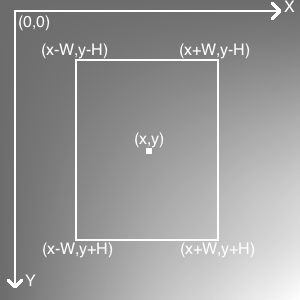
\includegraphics[scale=0.4]{./figs/integral_image}
%     \caption[Ejemplo de Imagen integral]{Ejemplo de Imagen integral: Representación de la ecuación \ref{eq:convolution_in_tree_operations}}
%    \label{fig:integral_image}                %% Etiqueta para la figura entera
% \end{figure}
% 
% \subsubsection{Simetrización}
% Para realizar la convolución a través de los bordes de las imagenes, se debe tener un cuidado especial para que no se produzcan efectos visuales no deseados y por consiguiente la detección de puntos de interés invalidos. Para esto, se consideran condiciones de borde simétricas, es decir que la imagen original es extendida simétricamente hacia cada uno de sus lados utilizando el tamaño del filtro caja más grande antes de calcular la imagen integral como se puede apreciar en la Fig. \ref{fig:symetrized_image}.
% \begin{figure}[tbhp]
%    \centering
%    %%----primera subfigura----
%    \subfloat[]{
%         \label{fig:lena}         %% Etiqueta para la primera subfigura
%         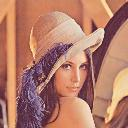
\includegraphics[scale=0.35]{./figs/lena}}
%    \hspace{0.1\linewidth}
%    %%----segunda subfigura----
%    \subfloat[]{
%         \label{fig:symetrized_lena}         %% Etiqueta para la segunda subfigura
%         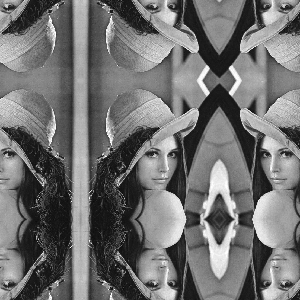
\includegraphics[scale=0.35]{./figs/symetrized_lena}}
%     \caption[Condiciones de borde simétricos para la imagen]{\ref{fig:lena}: Imagen de ``lena'' original. \ref{fig:symetrized_lena}:Imagen de ``lena'' extendida simétricamente}
%    \label{fig:symetrized_image}                %% Etiqueta para la figura entera
% \end{figure}
% 
% \subsubsection{Comparación con el espacio-escala Gaussiano}
% La representación espacio-escala de una imagen $u$ puede ser obtenida mediante la convolución con un kernel gaussiano como se aprecia en \ref{eq:convolution_scalar_space_kernel_gauss}
% \begin{equation}
% \label{eq:convolution_scalar_space_kernel_gauss}
% u_\sigma=g_\sigma * u
% \end{equation}
% donde $g_\sigma$ es el kernel gaussiano 2-D (centrado) que viene definido por \ref{eq:kernel_gaussiano_scale_space} y siendo $\sigma$ el parámetro que representa la escala.
% \begin{equation}
% \label{eq:kernel_gaussiano_scale_space}
% g_{\sigma}(x,y)=\frac{1}{2\pi\sigma^{2}}e^{-\frac{x^{2}+y^{2}}{2\sigma^{2}}}
% \end{equation}
% Haciendo uso de la técnica de filtros caja mencionados, la representación \ref{eq:kernel_gaussiano_scale_space} puede ser aproximada mediante la convolución discreta $\tilde{u}_{\sigma}=B_{L}*u$, donde $B_L$ es el filtro caja con ancho de banda $L$, esto es con un soporte cuadrado $\left[-\frac{L}{2},\frac{L}{2}\right]\times\left[-\frac{L}{2},\frac{L}{2}\right]$. En la configuración discreta, los valores tomados por $L$ son enteros e impares \cite{conf/scalespace/GwosdekGBW11}. Luego, los valores correspondientes a $\sigma$, vienen dados por \ref{eq:sigma_posible_values}.
% \begin{equation}
% \label{eq:sigma_posible_values}
% \sigma\text{\texttwosuperior=\ensuremath{\frac{L\text{\texttwosuperior-1}}{12}}}
% \end{equation}
% Observación: observar que el filtro caja debería ser normalizado por un factor $L^2$ para obtener un kernel cuadrado. Este no es el caso para tomar una consideración en lo que refiere a tiempos de cálculo. Esta normalización es llevada a cabo una sola vez durante el paso de detección de características.
% 
% En las figuras \ref{fig:japan_images} mostradas se puede observar la aproximación de escala-espacio obtenido cuando se usan filtros caja, comparado con la espacio escala lineal obtenida con los kernels gaussianos. Se debe observar que son similares, pero los espacio-escala aproximados exhiben algunos artefactos verticales y horizontales destacados debido a la anisotropía de los kernels caja.
% 
% \begin{figure}[tbhp]
%    \centering
%         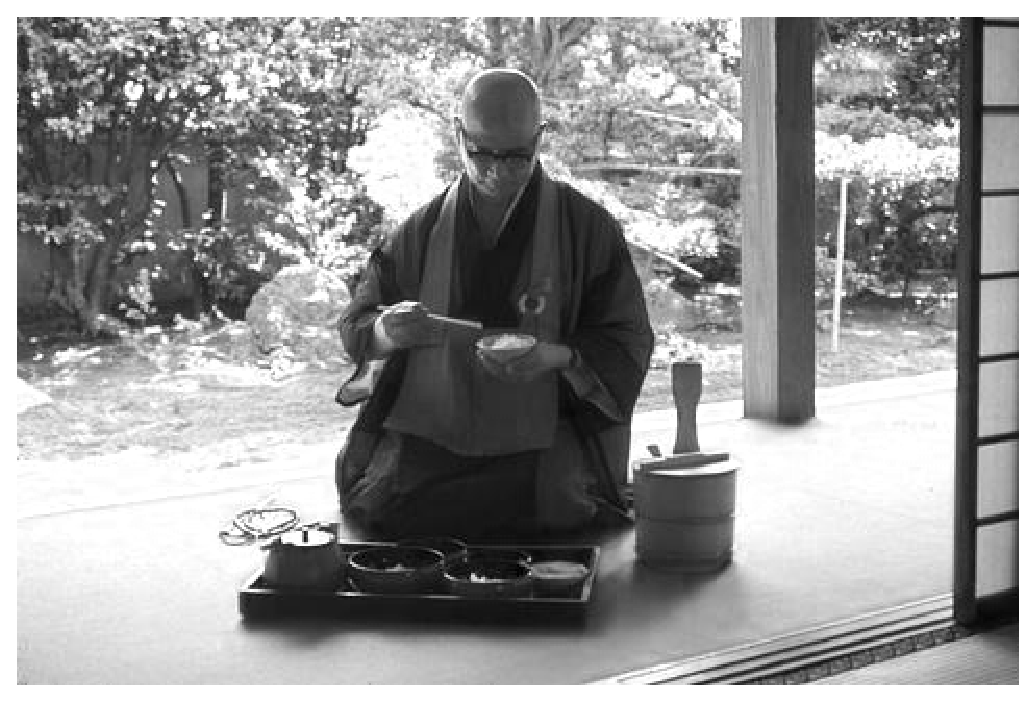
\includegraphics[scale=0.4]{./figs/japan}
%     \caption[Imagen original $u$]{Imagen original $u$}
%    \label{fig:japan_original_image}                %% Etiqueta para la figura entera
% \end{figure}
% 
% \begin{figure}[tbhp]
%    \centering
%    %%----primera subfigura----
%    \subfloat[]{
%         \label{fig:japan_tita}         %% Etiqueta para la primera subfigura
%         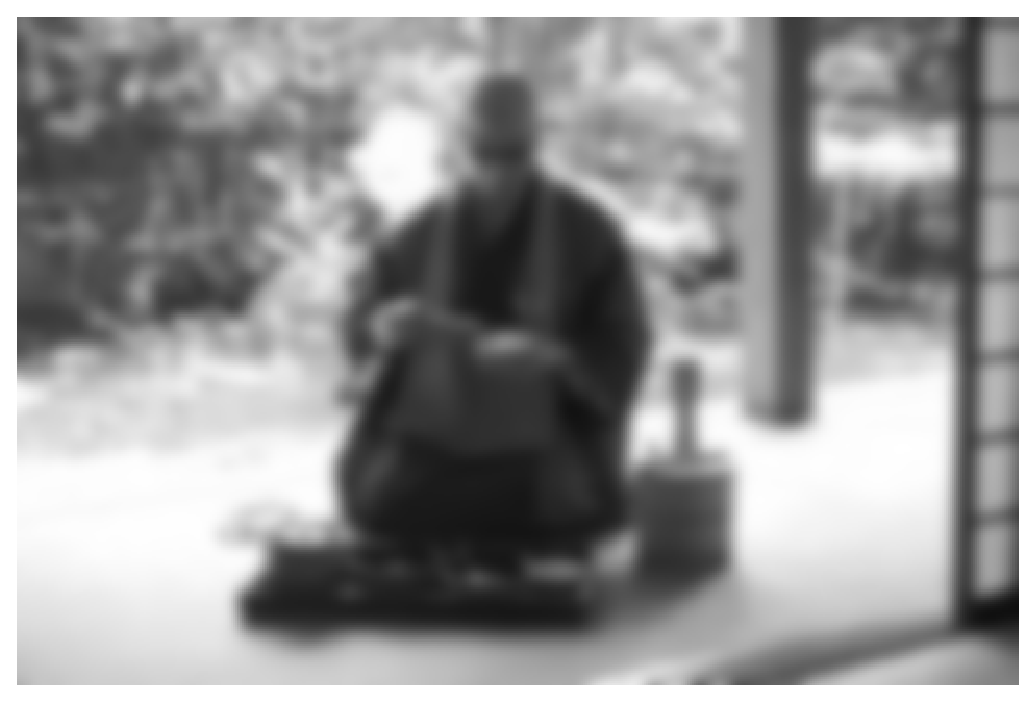
\includegraphics[scale=0.45]{./figs/japan_tita}}
%    %\hspace{0.01\linewidth}
%    %%----segunda subfigura----
%    \subfloat[]{
%         \label{fig:japan_tita_l}         %% Etiqueta para la segunda subfigura
%         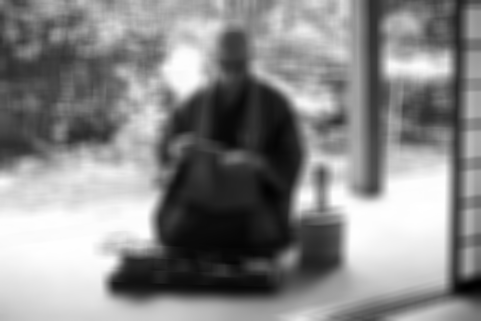
\includegraphics[scale=0.45]{./figs/japan_tita_l}}
%    \hspace{0.1\linewidth}
%    %%----tercera subfigura----
%    \subfloat[]{
%         \label{fig:japan_tita_1}         %% Etiqueta para la segunda subfigura
%         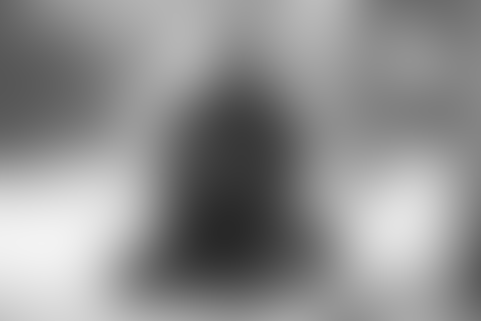
\includegraphics[scale=0.45]{./figs/japan_tita_1}}
%   % \hspace{0.01\linewidth}
%    %%----cuarta subfigura----
%    \subfloat[]{
%         \label{fig:japan_tita_1_l}         %% Etiqueta para la segunda subfigura
%         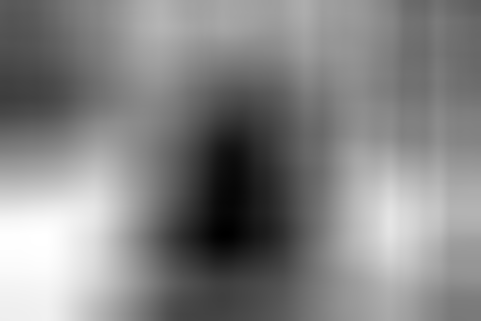
\includegraphics[scale=0.45]{./figs/japan_tita_1_l}}
%   %\hspace{0.01\linewidth}
%     \caption[caption]{Espacio-escala lineal obtenido con los kernels gaussianos y aproximación de espacio-escala cuando se usan filtros caja. (Se ha cambiado el contraste de la imagen para realzar los detalles). \ref{fig:japan_tita} $u_{\sigma}$ con $\sigma=1.708$, \ref{fig:japan_tita_l} $\tilde{u}_{\sigma}$ con $L=13$, \ref{fig:japan_tita_1} $u_{\sigma}$ con $\sigma=14.431$, \ref{fig:japan_tita_1_l} $\tilde{u}_{\sigma}$ con $L=101$}
% \label{fig:japan_images}                %% Etiqueta para la figura entera
% \end{figure}
% 
% Observación: Notar que una mejor aproximación de la escala-espacio puede obtenerse mediante el uso de filtros iterativo caja \cite{conf/scalespace/GwosdekGBW11}, pero el uso de los mismos implican una mayor complejidad.
% 
% \subsubsection{Muestreo escala-espacio}
% Similarmente al algoritmo SIFT, el análisis escala-espacio en SURF esta basado en un muestreo regular del parámetro de escala $\sigma$. La representación de la escala es dividida en \emph{octavas}: una nueva octava corresponde a la duplicación del tamaño del kernel (lo que significa que $\sigma$ sigue una serie geométrica). Cada octava es a su vez dividida en diferentes niveles (o intervalos), cada uno correspondiente al menor incremento del tamaño del filtro discreto involucrado.
% 
% Así definiendo $o$ como el índice que representa la octava e $i$ el índice del intervalo, el muestreo de escala es obtenido mediante la relación \ref{eq:relation_scale_octave}
% \begin{equation}
% \label{eq:relation_scale_octave}
% \sigma=\frac{1.2}{3}(2^{o}\times i+1)=\frac{1.2}{3}\times l,
% \end{equation}
% donde $3l$ es el ancho de banda del filtro caja correspondiente.
% 
% Notar que, contrariamente al método SIFT \cite{Lowe2004}, la imagen no es sub muestreada por un factor de dos en cada octava. No todas las escalas son usadas para seleccionar los puntos de interés y computar los descriptores correspondientes. Las escalas no utilizadas son requeridas para eliminar aquellos valores que no son máximos. Además, contrariamente al enfoque SIFT, el cálculo de la representación escala-espacio en sí no es necesaria, ya que los operadores diferenciales puede también aproximarse utilizando filtros de caja como se explaya a continuación en la sección \ref{subsubsection:approximation_diferential_operators}
% 
% \subsubsection{Aproximación de los operadores diferenciales}
% \label{subsubsection:approximation_diferential_operators}
% Con el objetivo de detectar los puntos interesantes y de construir los descriptores que incrementan los cambios de contraste afín, los operadores diferenciales de primer y segundo orden son calculados en el espacio escala. En la representación lineal espacio-escala, obtenida por la convolución con el kernel gaussiano (como se emplea en SIFT), esto se reduce a calcular la operación de convolución \ref{eq:operation_convolution_aproximation}
% \begin{equation}
% \label{eq:operation_convolution_aproximation}
% D_{\alpha\beta}^{(\sigma)}u_{0}(x,y,\sigma)=(D_{\alpha\beta}g_{\sigma})*u(x,y),
% \end{equation}
% donde $\alpha$ y $\beta$ se refieren a la primera o segunda variable ``x'' e ``y''.
% 
% En el método SURF, este cálculo es aproximado mediante la convolución de una combinación lineal de filtros caja \ref{eq:combination_filter_box}
% \begin{equation}
% \label{eq:combination_filter_box}
% \tilde{D_{\alpha\beta}^{(\sigma)}*u,}
% \end{equation}
% definido en los párrafos siguientes.

% \section{Correspondencia de características entre imágenes}
% \label{sec:correspondencia_caracteristicas_img}
% La correspondencia de características es el proceso en el que los descriptores de los puntos claves de dos o más imágenes son comparados y los pares de correspondencias son creados. Existen muchos métodos para realizar la correspondencia de descriptores de puntos claves. El método más básico está basado en la búsqueda del vecino más cercano entre dos conjuntos de puntos claves. Dadas dos imágenes $I_1$ e $I_2$, el espacio vector n-dimensional se encuentra formado por los descriptores $d(k)$ del conjunto $K1$, $K2$ de puntos claves. Los pares de correspondencias $<k_{i},l_{i}>$ se forman como lo expresa la expresión \ref{eq:correspondence_pairs:expr}
% \begin{equation}
%  \label{eq:correspondence_pairs:expr}
% \forall k_{i}\in K_{1}:l_{i}=\arg\min_{l\in K_{2}}|d(k_{i})-d(l)|
% \end{equation}
% 
% %http://saravananthirumuruganathan.wordpress.com/2010/05/17/a-detailed-introduction-to-k-nearest-neighbor-knn-algorithm/
% % \subsection{esquema de búsqueda en árbol kd}
% % slipa modificado por mi
% % La idea general detrás de los árboles KD se describirá a continuación. Los elementos guardados en el árbol KD son vectores de altas dimensiones en $R^d$. En el primer nivel (la raíz) del árbol, los datos son divididos en dos mitades por un hiper plano ortogonal a una dimensión elegida con un valor de umbral. Generalmente, esta división sea realiza se realiza con la media en la dimensión con la mayor varianza del conjunto de datos. Mediante la comparación del vector de consulta con el ``valor de partición'', es fácil determinar a que mitad de el conjunto de datos del vector de consulta pertenece. Cada una de las mitades de los datos, es luego recursivamente dividida de la misma forma explicada anteriormente para crear un árbol binario completamente balanceado.
% % En la parte inferior del árbol, cada nodo del árbol, corresponde a un punto simple del conjunto de datos, aunque en algunas aplicaciones, los nodos hojas pueden tener más de un punto.
% % La profundidad del árbol resulta ser $log_2 (N)$ donde $N$ es el número de puntos del conjunto de datos.
% 
% % Dado un vector de consulta, un descenso en el árbol requiere $log_2(N)$ comparaciones y el acceso a un nodo hoja del arbol.
% Una vez que han sido identificados los puntos claves y sus descriptores asociados sobre la imagen, % utilizando las herramientas descriptas en la sección %(\ref{extraccion_caracteristicas}), 
% se procede con la búsqueda de correspondencia (en caso de existir) entre la imagen de entrenamiento o patrón y la imagen del flujo de vídeo. De esta forma se busca identificar si el objeto se encuentra presente en la imagen capturada.
% 
% Como se ha visto, un descriptor SURF es un vector de 64 dimensiones que caracteriza localmente una vecindad de un punto clave. Generalmente, gran cantidad de descriptores SURF son extraídos de la imagen y la consulta consiste en buscar los vectores que mejor coincidan, tarea que no resulta trivial a la hora de lograr tiempos de ejecución acotados.
% Existen diversas técnicas, para dar respuestas a este problema. Una de más mencionadas es la denominada \textit{búsqueda del vecino más cercano} (del ingl\'es, Nearest Neighbor Search o NNS) \cite{AryaEtAl98} y sus variantes.

% \subsection{Búsqueda del vecino más cercano}
% El m\'etodo de búsqueda del vecino más cercano es de utilidad en gran variedad de aplicaciones como el reconocimiento de imágenes, la compresión de datos, el reconocimiento de patrones y su clasificación, el aprendizaje máquina, los sistemas de recuperación de documentos, estadísticas y análisis de datos, entre otros. 
% 
% Es un problema de optimización que intenta buscar los puntos más cercanos en un espacio métrico. Éste, puede definirse de la siguiente forma: dado un conjunto de puntos $P=\left\{ p_{1,...,}p_{n}\right\}$ en un espacio métrico $M$ y un punto de consulta $q \in M$, encontrar el/los punto/s más cercano/s a $q$ en $P$ donde $M$ es un espacio euclídeo d-dimensional y las distancia es medida mediante la distancia euclídea o Manhattan. 

% Resolver este tipo de problemas no resulta trivial en espacios de grandes dimensiones. No es usual encontrar algoritmos que posean un rendimiento mayor al de la búsqueda lineal (también conocida como ``búsqueda por fuerza bruta''), la cual resulta ser muy costosa y a veces inaplicable para muchas aplicaciones. Es por esto, que se ha generado un gran interés en algoritmos \footnote{\url{http://www.cs.umd.edu/~mount/ANN/}} que puedan realizar la búsqueda del vecino más cercano de forma aproximada, con lo cual es posible lograr mejoras significativas en tiempo de ejecución con errores de precisión relativamente pequeños y aceptables \cite{Beis:1997:SIU:794189.794431}.

% \subsubsection{Remoción de pares irrelevantes}
% Esta aproximación tiene la desventaja que la correspondencia se genera para cada $k_i$, independientemente de que las características sean muy similares, debido a que siempre se encuentra un vecino cercano. Lowe \ref{Lowe2004} propone usar un ratio para rechazar pares de puntos claves no especificos. La distancia euclidea $d1$, $d2$ de dos vecinos más cercanos es comparada y si el ratio cumple $\frac{d_{1}}{d_{2}}>\varepsilon\qquad(\varepsilon=0.8\:\ref{Lowe2004})$, el par de correspondencias es desechado. Esto rechaza todos los puntos claves, para los cuales no hay una correspondencia especifica en la segunda imagen.
% 
% En muchos casos el objeto plano buscado contiene muchas características genericas como esquinas o simples curvas. Este problema ocurre comunmente cuando se buscan locos o simple logos. Estas características pueden ser encontradas muchas veces en la imágen objetivo y pueden producir que no se encuentre la homografía correcta. Esta remoción reduce el numero de pares dispnibles para buscar la correspondencia, pero realza la habilidad de buscar la homografía correcta mediante la reducción de correspondencias incorrectas.

% \section{Correspondencia de los puntos claves}
% 
%  \subsection{Indexación rápida}
% %ESTO NO SE USA!! : PORQUE SEG;UN LO QUE ME MANDO MARIUS MUJA EN EL MAIL DICE QUE DIVIDIR SEGUN EL SIGNO ES MUCHO MAS LENTO Y LOS RESULTADOS NO SON APRECIABLES.
%  Comúnmente, los puntos claves detectados, se hallan en regiones y puntos que difieren en intensidad de su vecindad. El signo del Laplaciano (por ejemplo la traza de la matriz hessiana) distingue regiones de claras (alta luminosidad) de fondos oscuros (baja luminosidad) y viceversa. Este dato está disponible sin un costo computacional extra debido a que ya ha sido calculada en la fase de detección descripta en la Sec. \ref{sec:matHessiana}. Así, en la etapa de búsqueda de correspondencias, solo se comparan las características si el ``contraste'' entre ellas es similar, véase la figura \ref{fig:contrastcomparation} como un ejemplo. Esta información resulta ventajosa para métodos de indexación como kd-trees definiendo un hiper plano para dividir los datos, opuesto a seleccionar un elemento aleatoriamente o usar estadísticas de características.
% 
%     \begin{figure}[tbhp]
%       \centering
% 	    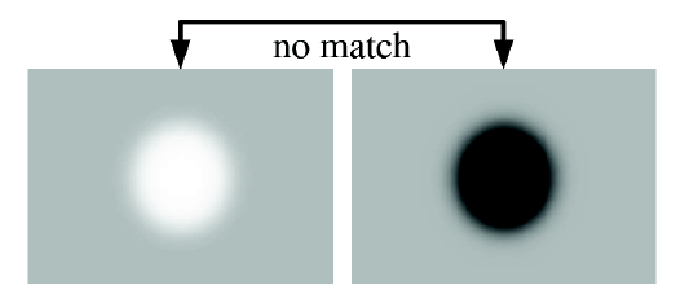
\includegraphics[scale=0.4]{./figs/notmatching}
% 	\caption[]{Si el contraste entre dos puntos de interés es diferente (oscuro sobre fondo claro versus claro sobre fondo oscuro), el candidato no es considerado como una coincidencia valiosa.)}
%       \label{fig:contrastcomparation}
%     \end{figure}

 %Este umbral puede ser interpretado como: Un par es detectado como coincidente si la distancia es lo suficientemente cercana a $n$ veces la distancia del segundo más cercano.